\documentclass[a4paper,11pt]{article}
\usepackage[left=1.5cm, right=1.5cm, top=2cm, bottom=1.5cm]{geometry}
\usepackage{graphicx}
\usepackage{amssymb}
\usepackage{amsmath}
\usepackage{wrapfig}

\newcommand{\parallelsum}{\mathbin{\!/\mkern-5mu/\!}}

\begin{document}
\title{\LARGE{\textbf{ECEN 204 Design Report}\\Pre-Amplifier}}
\author{Niels Clayton : 300437590}
\date{October 9$th$, 2019}
\maketitle
\hrule

\section{Introduction}

The role of the pre-amplifier is to amplify a low voltage electrical signal (usually within the millivolt range) to a signal of voltage large enough for further processing, usually power amplification.  The design of our pre-amplifier must be able to operate from a 9V power supply, and offer a gain of at least 5 across the audible spectrum. 

\section{Design}

\begin{wrapfigure}{r}{0.4\textwidth}
\vspace{-40pt}
\begin{center}
\fbox{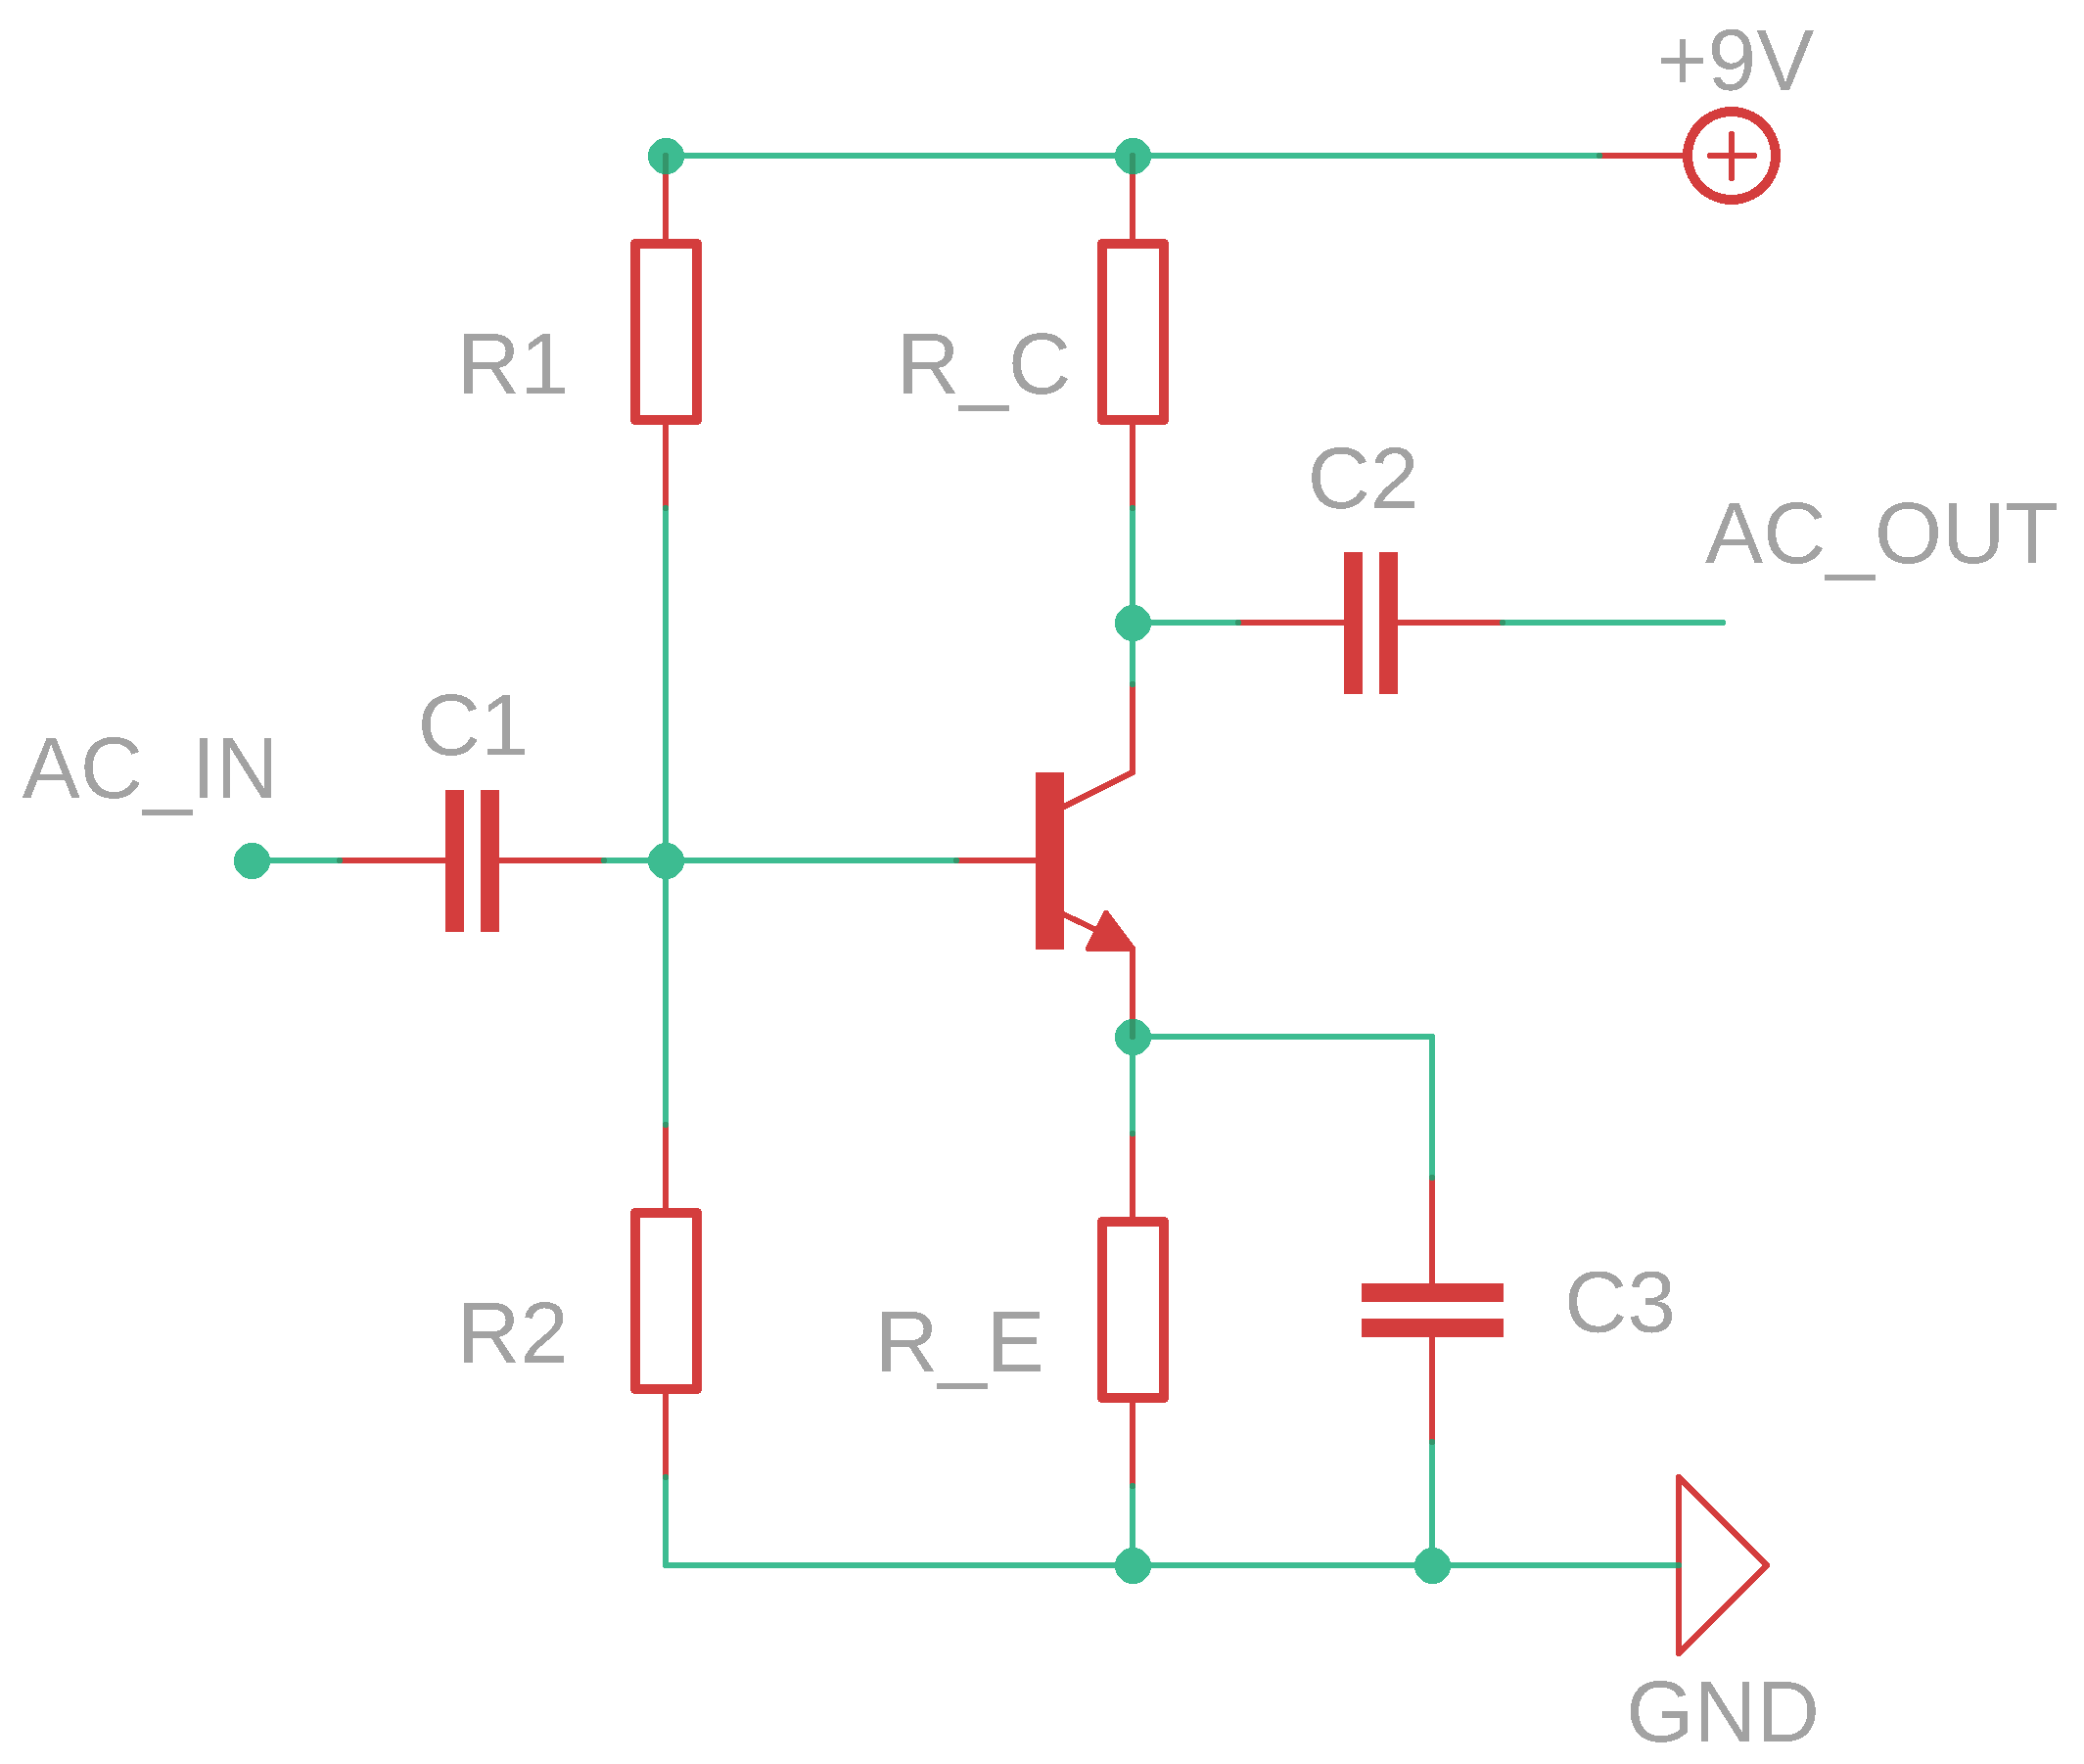
\includegraphics[width=0.4\textwidth]{design.png}}
\end{center}
\vspace{-18pt}
\caption{Base Pre-amplifier Design}
\end{wrapfigure}

The basic circuit design of the pre-amplifier can be seen in figure 1. This amplifier will utilise a BC547 transistor in a common emitter configuration. The base of the transistor will be connected to the 9V power rail through a voltage divider, allowing for the selection of the initial operating point (q-point) of the transistor.\\\\

The gain of this amplifier is dependant on the ratio of the collector resistor ($R_C$) to the emitter resistor ($R_E$). since we are aiming for a gain of at least 6, we must chose resistors that will provide this. in this circuit we will use a resistor value of $6k \Omega$ for $R_C$, and $1k \Omega$ for $R_E$.\\

$$ Gain = \frac{R_C}{R_E} = \frac{6k}{1k} = 6 $$\\

Now that we have values for $R_C$ and $R_E$ that will give us a gain of 6, we want to calculate the values of $R1$ and $R2$ that will place the transistor q-point at 4.5 volts with no input AC signal. this will allow for the maximum amplification of the input signal, with equal spacing of 4.5V on possible on either side of the q-point.

$$I_C = \frac{V}{R_C} = \frac{4.5V}{6k} = 0.75mA$$
$$V_C = I_C \times R_E = 1k \Omega \times 0.75mA = 0.75V$$
$$V_B = V_C + V_{BE} = 0.75V + 0.7V = 1.45V$$

\pagebreak

With out calculated base voltage of the transistor, we can look at $R1$ and $R2$ as a simple voltage divider. By choosing a value of $10k \Omega$ for $R2$ we can calculate a value of $R1$ to be $ 52k \Omega$. \\

Now that the values of all resistors have been selected, the values of capacitors $C1$ and $C3$ must be selected. Since $C2$ is purely a DC filter, we can chose any available capacitor size, in our case a $10\mu F$ cap.\\

Calculating $C_1$:

\begin{align*}
  C_1 &= \frac{1}{2 \pi f_c R} \\
          &= \frac{1}{2\pi\times 2\times 8387} \\
          &=9.4 \mu F \\
          C_{1} &= 10\mu F
\end{align*}

With values $f_c = \frac{1}{10} \times$ target frequency, and $R = R_1 \parallelsum R_2$.\\

Calculating $C_2$:

\begin{align*}
    C_{3} &= \frac{1}{2\pi f_{c}r_{e}'} \\
          &= \frac{1}{2\pi \times 20Hz\times 33\Omega} \\
          &= 238\mu F \\
          C_{3} &= 100\mu F
\end{align*}

With values: $$r_e ' = \frac{1}{40\times I_C} = \frac{1}{40\times 0.75mA} = 33\Omega$$\\

With these calculations, we come to the final complete design seen below in figure 2.

\begin{figure}[h]
 \begin{center}
  \fbox{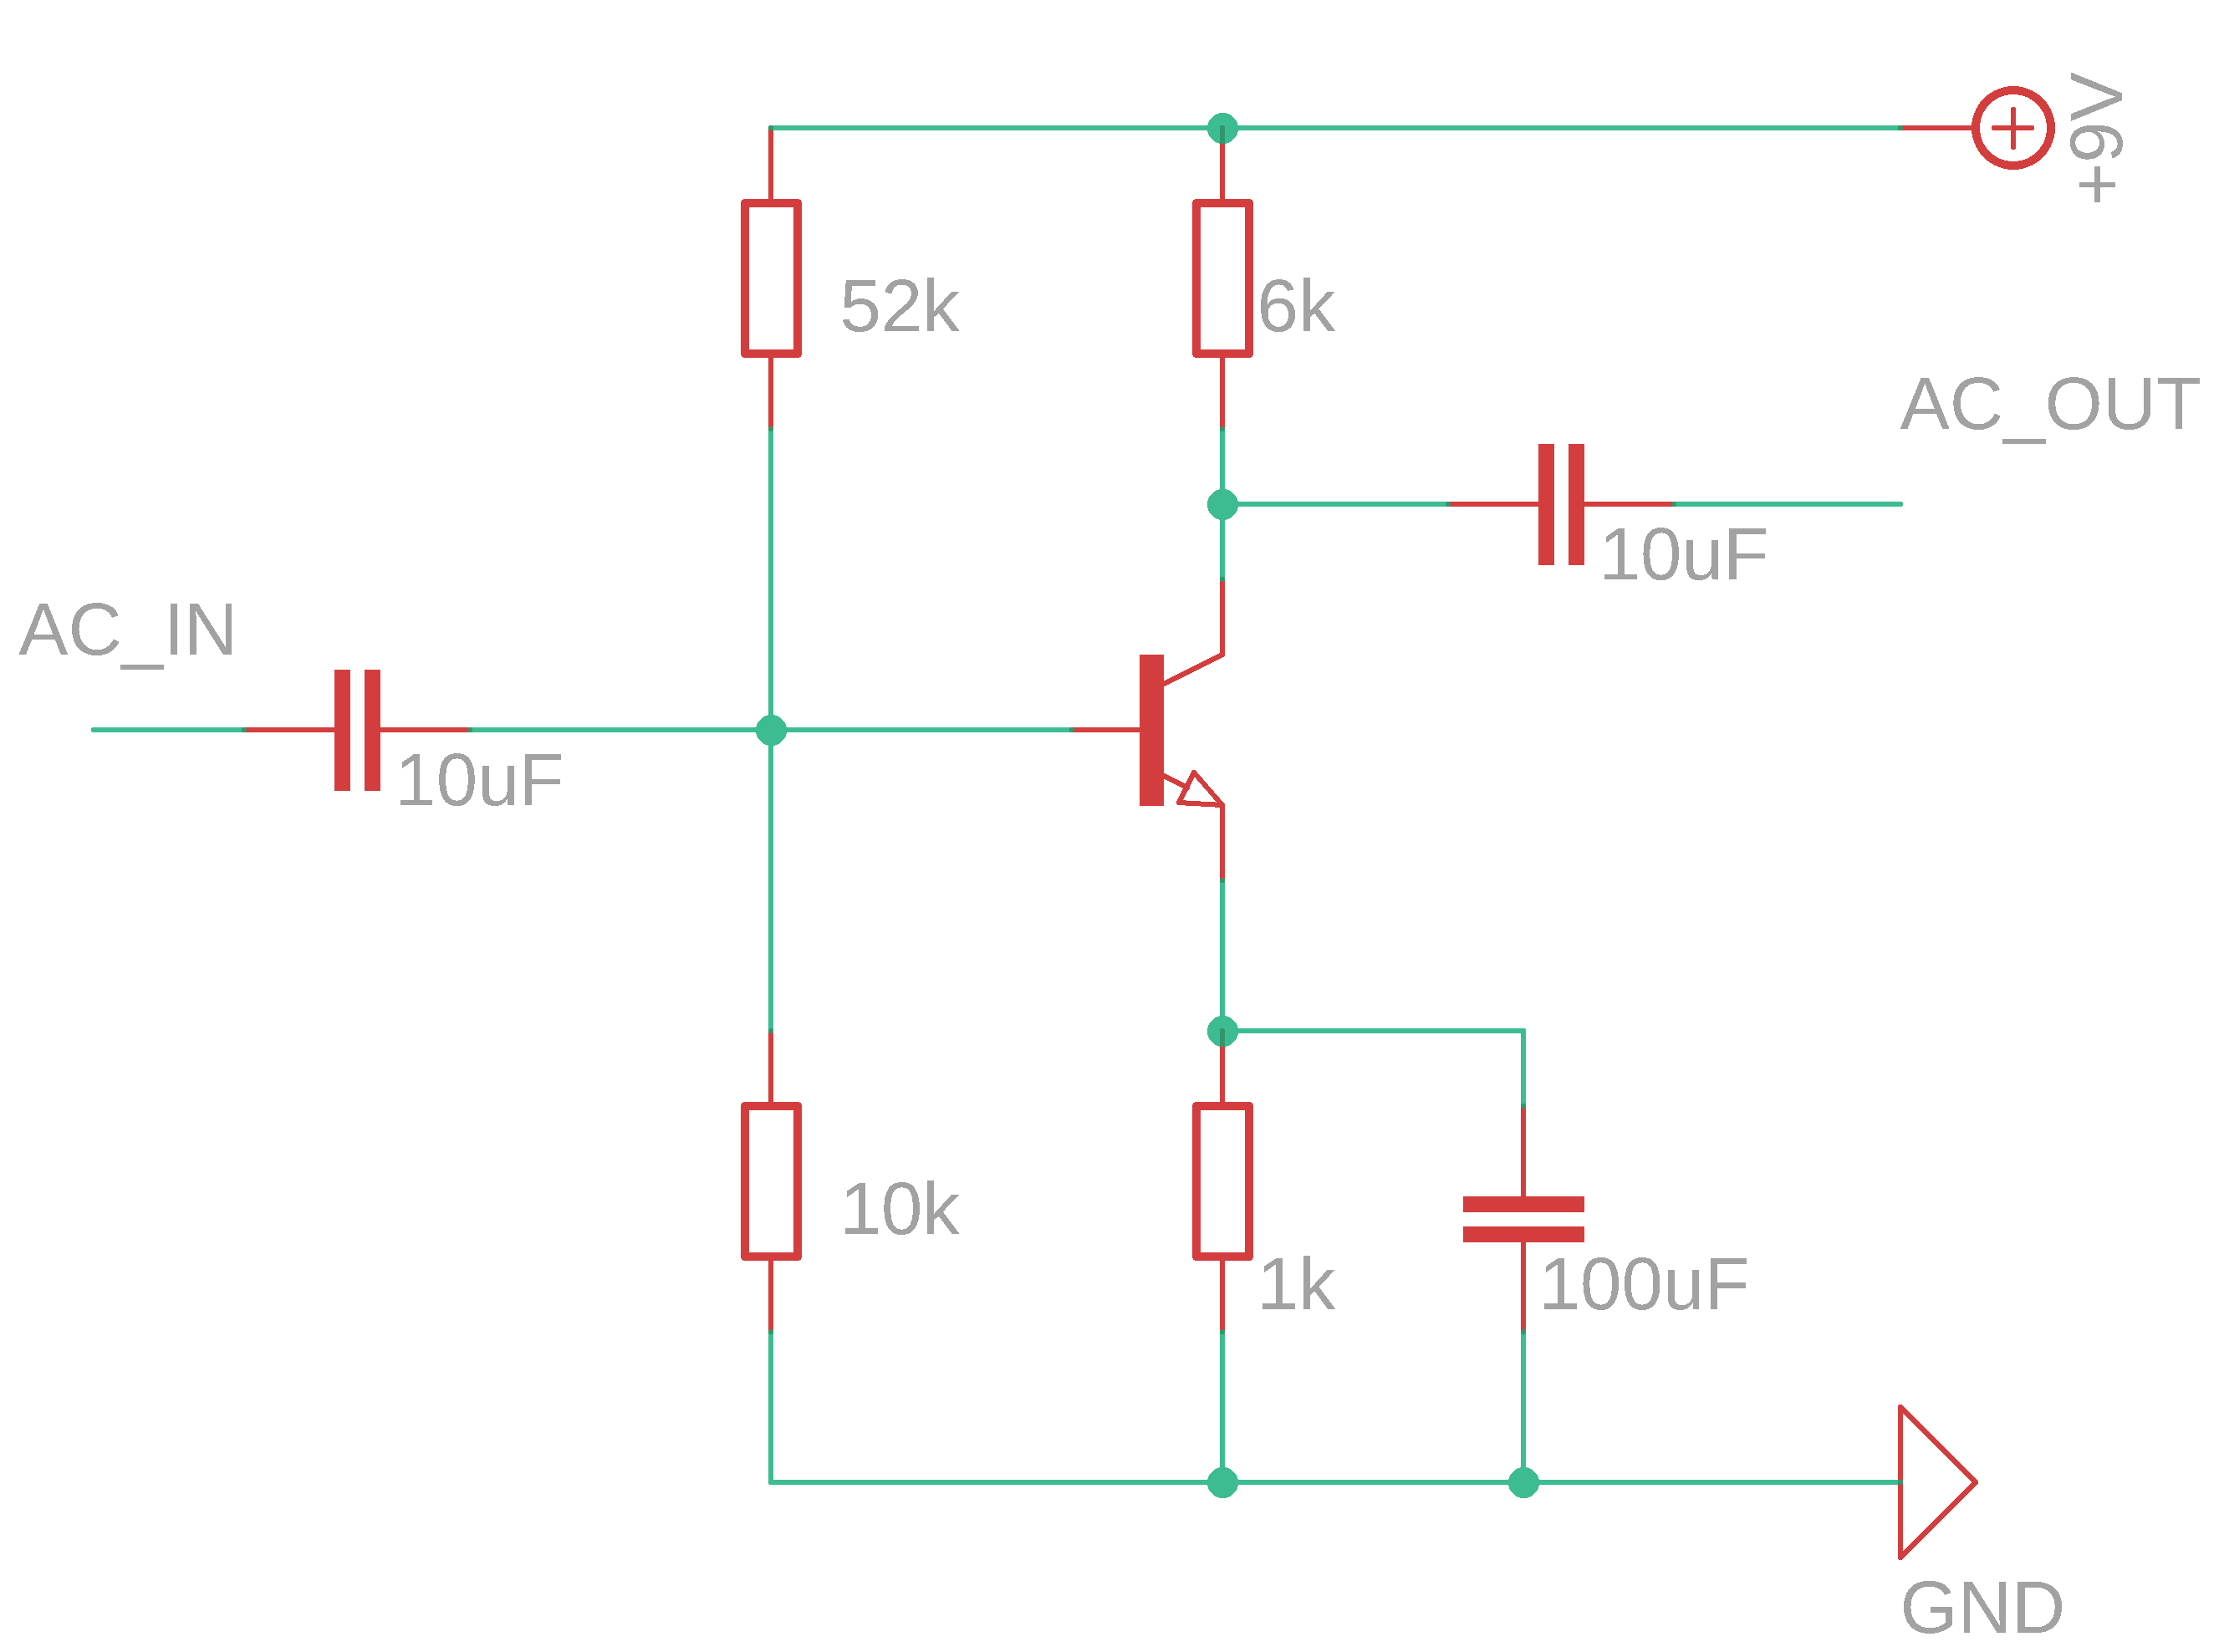
\includegraphics[width = 0.7\textwidth]{final.png}}
  \vspace{-8pt}
  \caption{Finalised circuit design with component values}
  \vspace{-15pt}
 \end{center}
\end{figure}

\pagebreak

The design of the circuit shown in figure 2 has some trade-offs that become more apparent when operating the circuit, mainly its non-adjustable q-point, the constant power draw of the circuit, and the phase offset of 180$^o$ on the output signal compared to the input. 
 
\section{Prototyping, Construction and testing } 

\begin{wrapfigure}{r}{0.4\textwidth}
\vspace{-40pt}
\begin{center}
\fbox{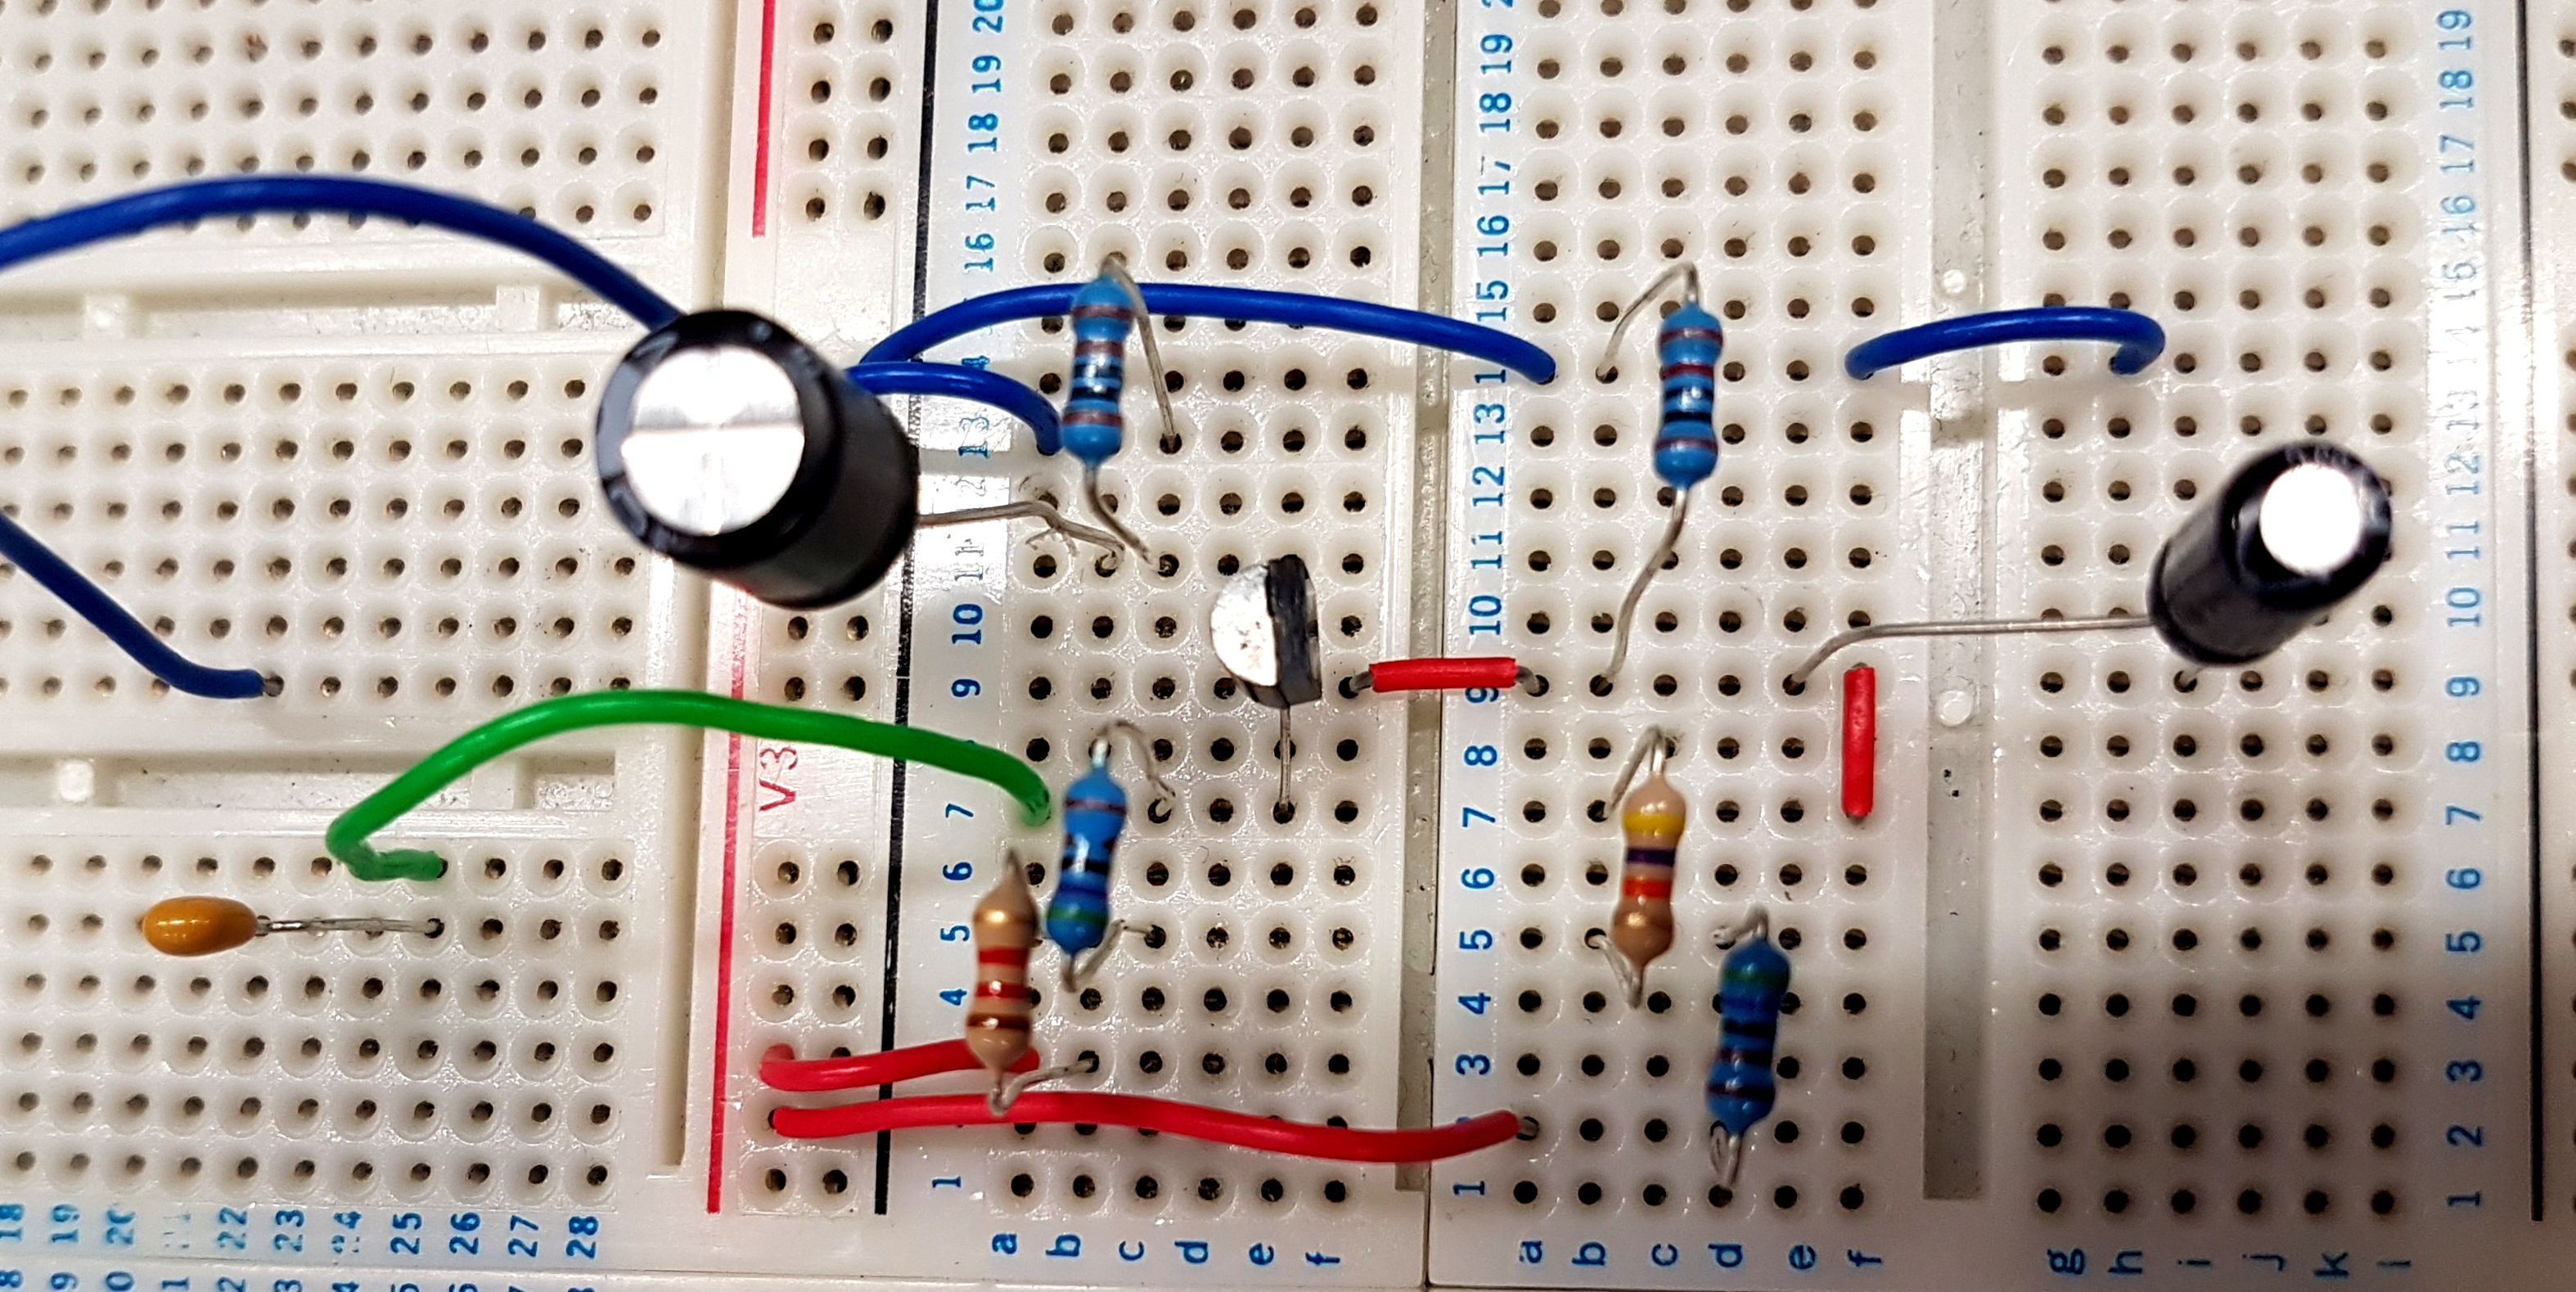
\includegraphics[width=0.4\textwidth]{breadboard.jpg}}
\end{center}
\vspace{-8pt}
\caption{Breadboard prototyping of the pre-amplifier circuit}
\end{wrapfigure}

Now that we have the overall design of the pre-amplifier, the circuit was prototyped and tested on breadboard, and simulated in LTSpice to backup the results that were achieved on breadboard. Since the brief dictates that the pre-amplifier have a gain of atleast 5 across the audible spectrum before the instillation of the bypass capacitor ($C_3$),  our circuits performance was tested for a range of frequencies between 20$Hz$ and 20$kHz$. \\\\


\begin{wrapfigure}{r}{0.4\textwidth}

\begin{center}
\vspace{-8pt}
\fbox{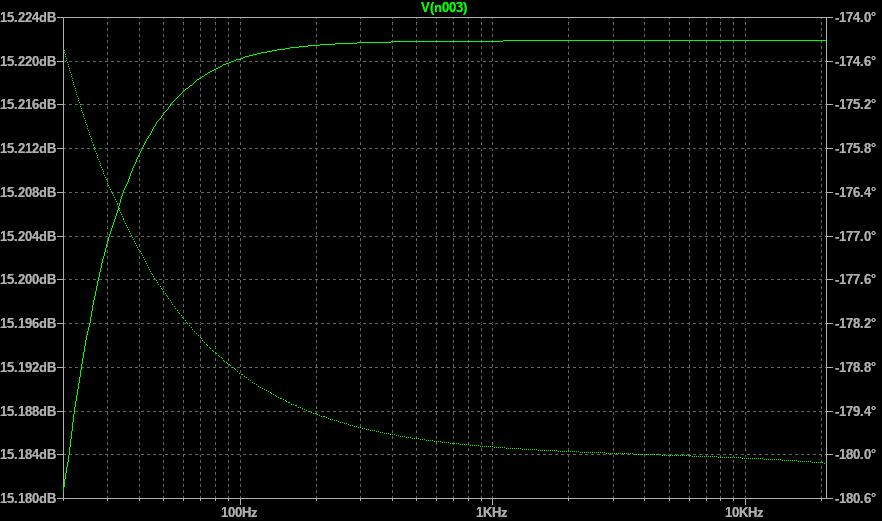
\includegraphics[width=0.45\textwidth]{frequency1.jpg}}
\end{center}
\vspace{-8pt}
\caption{Frequency response of pre-amp without bypass cap simulated in spice}
\vspace{-3cm}
\end{wrapfigure}

Frequency response of the pre-amplifier circuit before bypass capacitor:\\
\begin{tabular}{|c|c|c|c|c|}  
\hline
Frequency &\(\displaystyle V_{Pk-Pk}in\)  & \(\displaystyle V_{Pk-Pk} out\) & Gain & Power draw\\
\hline
20\(\displaystyle Hz \) & 200\(\displaystyle mV\)     &  990\(\displaystyle mV\)  & 4.9    & 8.37 \(\displaystyle mW\)\\
40\(\displaystyle Hz \) &  200\(\displaystyle mV\)    &  1.07\(\displaystyle V\)    & 5.35  & 8.37 \(\displaystyle mW\)\\
60\(\displaystyle Hz \) &  200\(\displaystyle mV\)    & 1.14\(\displaystyle V\)     & 5.7    & 8.37 \(\displaystyle mW\)  \\
80\(\displaystyle Hz \)&  200\(\displaystyle mV\)     &  1.14\(\displaystyle V\)    & 5.7    & 8.37 \(\displaystyle mW\)\\
100\(\displaystyle Hz \)&  200\(\displaystyle mV\)  &  1.14\(\displaystyle V\)     & 5.7    & 8.37 \(\displaystyle mW\) \\
1\(\displaystyle k Hz \)&  200\(\displaystyle mV\)    &  1.14\(\displaystyle V\)     & 5.7    & 8.37 \(\displaystyle mW\)\\
20\(\displaystyle k Hz \)& 200\(\displaystyle mV\)   &  1.14\(\displaystyle V\)    & 5.7    & 8.37 \(\displaystyle mW\) \\
\hline
\end{tabular}\\\\


It can be observed from the table above that our designed amplifier circuit meets all of the required specification of the circuit, maintaining a near constant gain of 5.7 times the input signal voltage except for frequencies less than 40$Hz$, with a lowest gain of 4.9. This dip in gain below the expected 5 at 20$Hz$ is most likely due to the tolerances of the components used within the circuit, causing there to be small discrepancies between what we expect from the circuit, and what is achieved. These values that were taken within the lab are also corroborated by the AC sweep simulations run in LTSpice that can be seen in figures 4 and 5. \\


\begin{wrapfigure}{r}{0.4\textwidth}

\begin{center}
\fbox{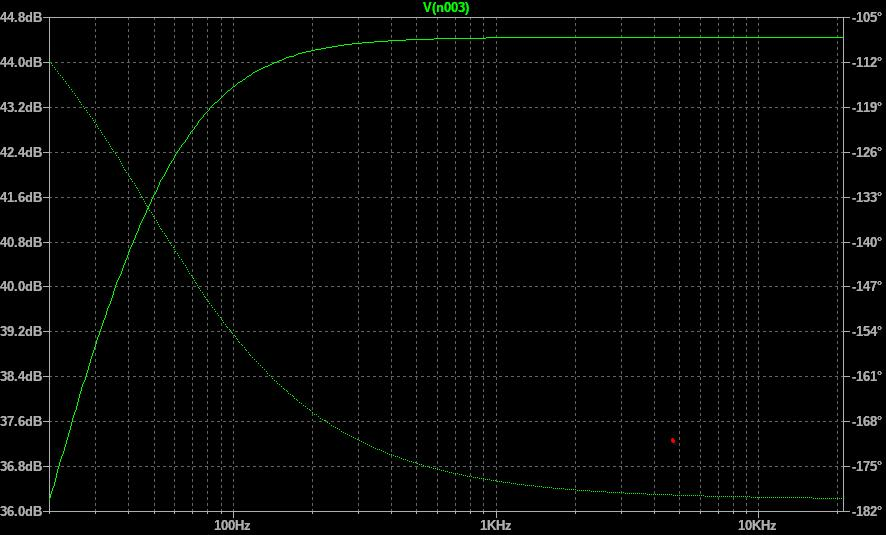
\includegraphics[width=0.45\textwidth]{frequency.jpg}}
\end{center}
\vspace{-8pt}
\caption{Frequency response of pre-amp with bypass cap simulated in spice}
\vspace{-7cm}
\end{wrapfigure}

Frequency response of the pre-amplifier circuit after bypass capacitor:\\
\begin{tabular}{|c|c|c|c|c|}  
\hline
Frequency &  \(\displaystyle V_{Pk-Pk}in \)  & \(\displaystyle V_{Pk-Pk} out\) & Gain & Power draw\\
\hline
20\(\displaystyle Hz \) & 30\(\displaystyle mV\)     &  1.56\(\displaystyle V\)  & 52    & 8.37 \(\displaystyle mW\)\\
40\(\displaystyle Hz \) &  30\(\displaystyle mV\)     &  2.98\(\displaystyle V\)    & 99.3  & 8.37 \(\displaystyle mW\)\\
60\(\displaystyle Hz \) &  30\(\displaystyle mV\)    & 3.8\(\displaystyle V\)     & 126.6    & 8.37 \(\displaystyle mW\)  \\
80\(\displaystyle Hz \)&  30\(\displaystyle mV\)       &  4.2\(\displaystyle V\)    & 140    & 8.37 \(\displaystyle mW\)\\
100\(\displaystyle Hz \)&  30\(\displaystyle mV\)    &  4.48\(\displaystyle V\)     & 149.3    & 8.37 \(\displaystyle mW\) \\
150\(\displaystyle Hz \)&  30\(\displaystyle mV\)    &  4.8\(\displaystyle V\)     & 160    & 8.37 \(\displaystyle mW\) \\
1\(\displaystyle k Hz \)&  30\(\displaystyle mV\)     &  5.1\(\displaystyle V\)     & 170   & 8.37 \(\displaystyle mW\)\\
20\(\displaystyle k Hz \)& 30\(\displaystyle mV\)     &  5.12\(\displaystyle V\)    & 170.6    & 8.37 \(\displaystyle mW\) \\
\hline
\end{tabular}

\pagebreak

Now that we have tested and observed that our design meets the specifications required, we can transfer our final design from breadboard to perf-board, soldering all of the required components in place. This final design can be seen below in figure 6. 

\begin{figure}[h]
 \begin{center}
  \fbox{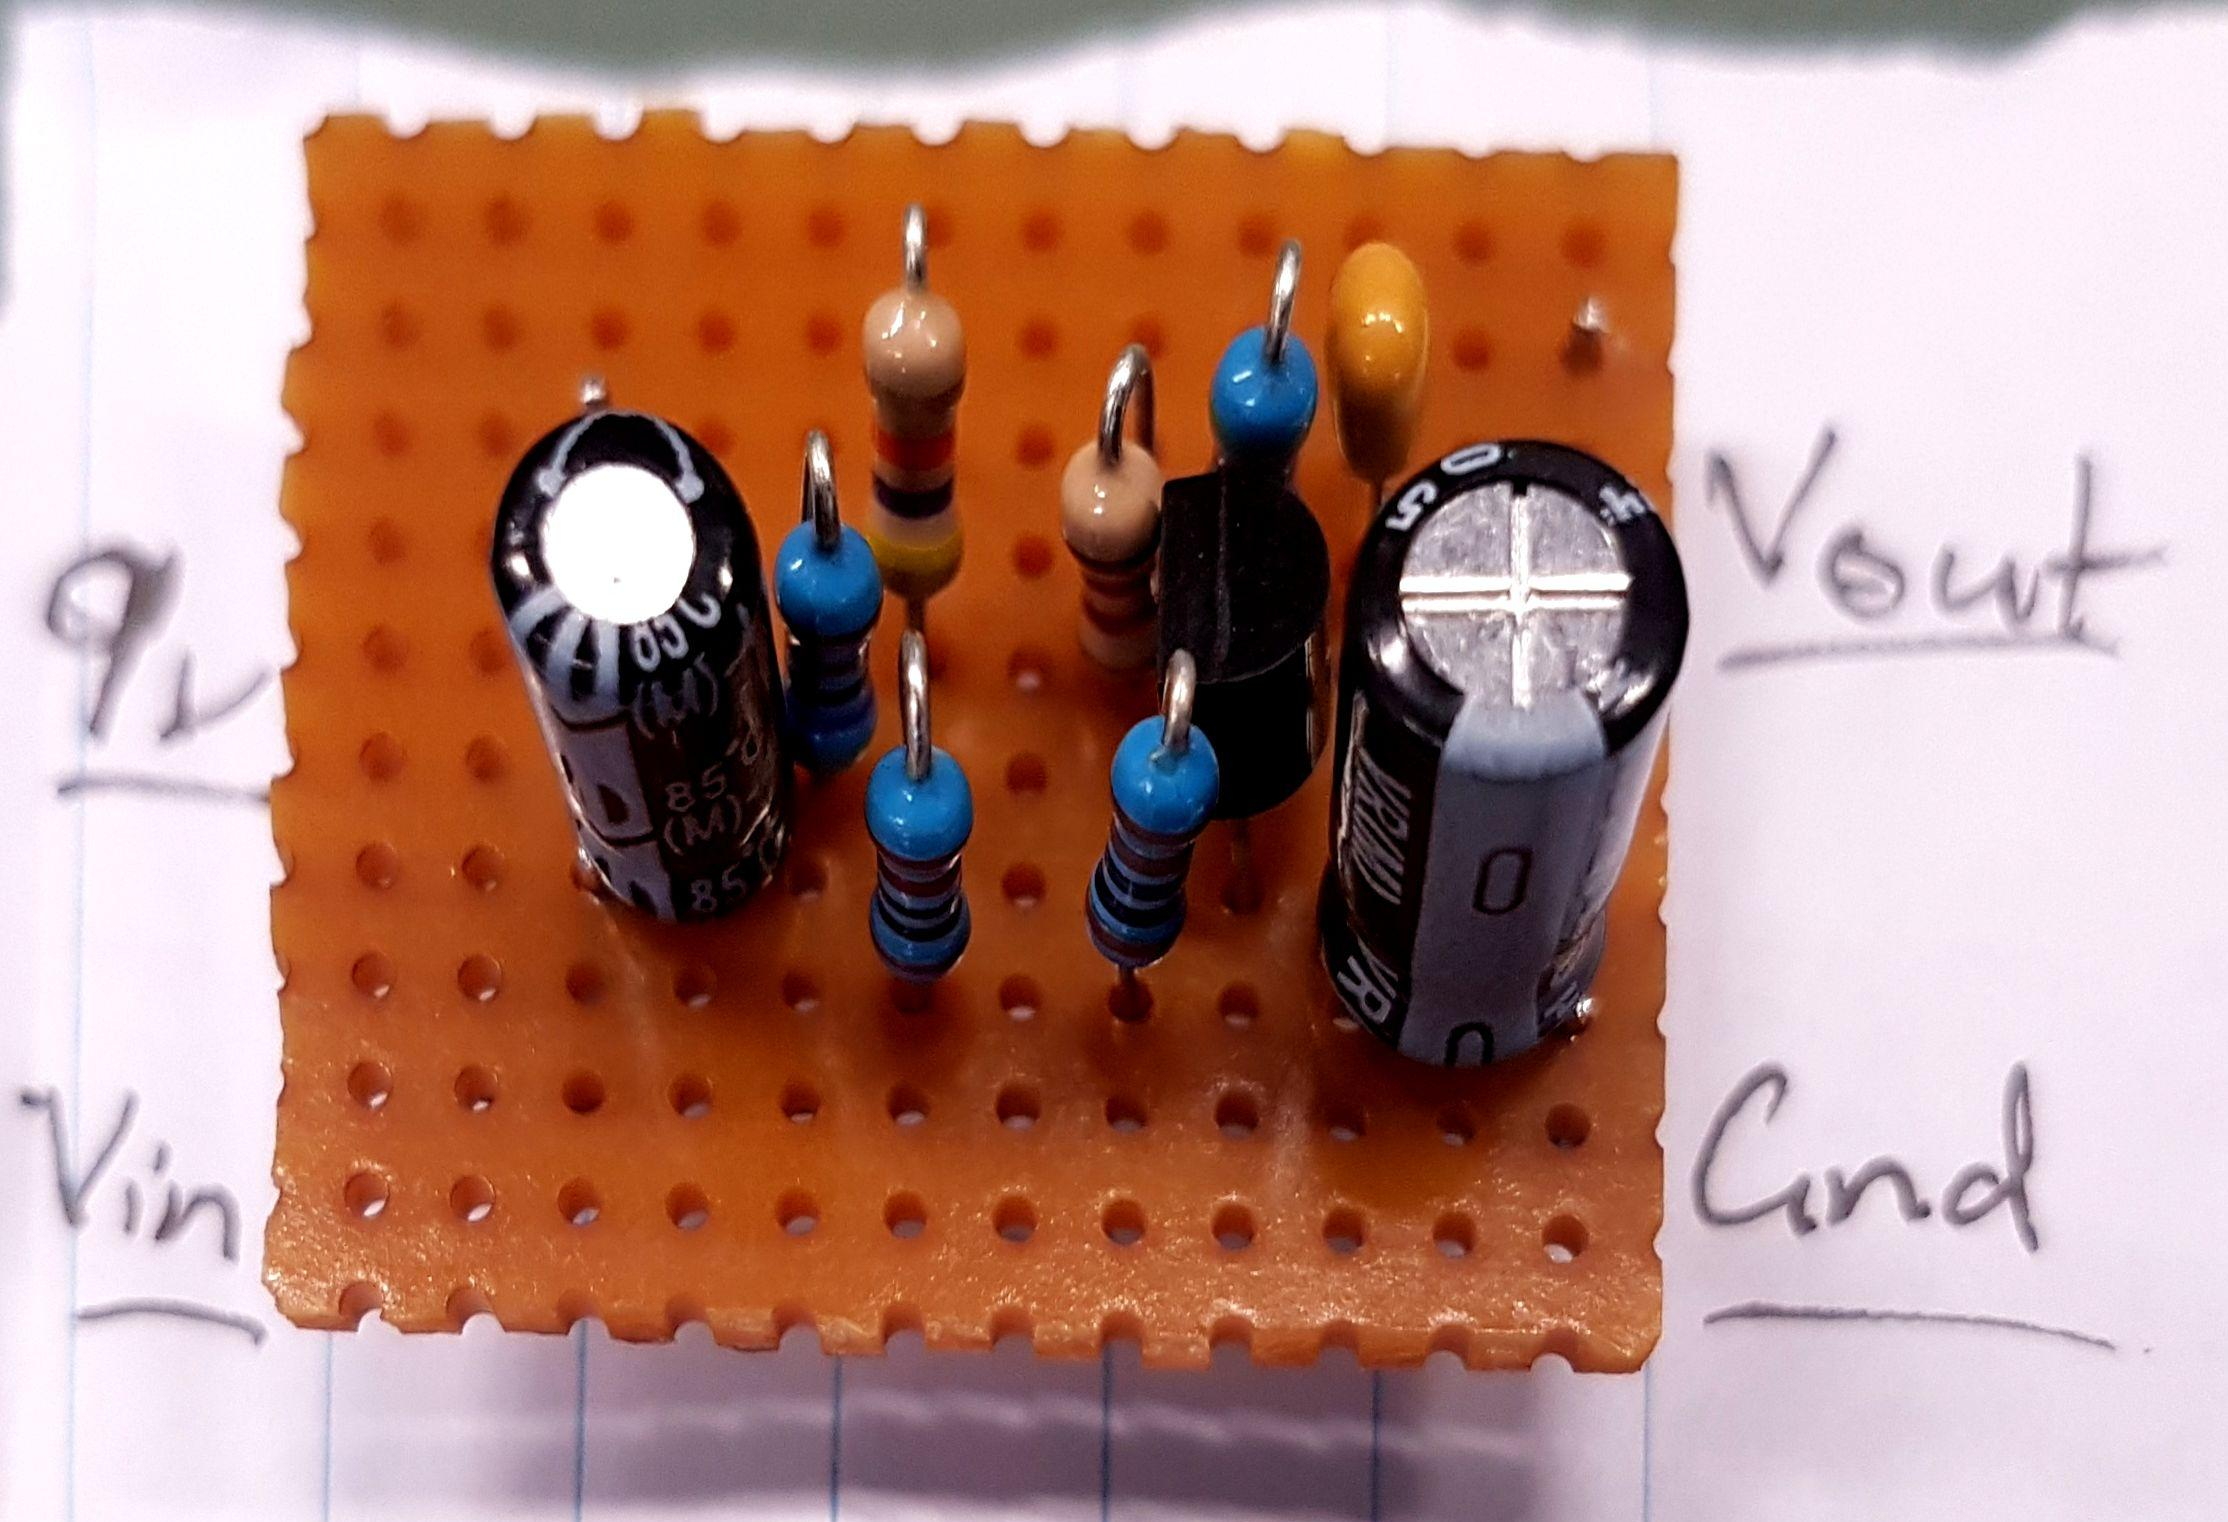
\includegraphics[width = 0.7\textwidth]{perfboard.jpg}}
  \caption{Final pre-amplifier circuit built on perf-board}
 \end{center}
\end{figure}

\section{Discussion}

Overall, our final design for the pre-amplifier met all of the required specifications. The only design issue encountered in this project was the lack of resistor values that exactly matched the required values calculated. This was remedied by using combinations on resistors within the final design to more accurately recreate the desired.
Overall this design meets the required specifications, however there are many ways in which it can be improved, most importantly would be the addition of a moveable q-point value. This could be done by making the R1 resistor a variable resistor, which will alter the current into the base, and thereby the q-point. 


This design project was overall very enjoyable, and interesting, however it was very difficult to design the pre-amplifier in our assigned lab time because the lectures on the subject had not yet been covered. Because of this we were forced to come into other lab sessions in-order of complete our design.

\section{Additional questions}

a).

The purpose of the input capacitor is to super-impose the input AC signal onto the DC voltage between resistors R1 and R2. 

The purpose of the output capacitor is to remove the DC offset from the  output of the the circuit.

The purpose of the bypass capacitor is to further amply the signal. this is done by decreasing the overall resistance of the emitter side of the transistor, and thereby increasing the gain of the circuit since gain is determined by the ratio of $R_C$ to $R_E$. 

\pagebreak

\section{Appendix} 

\begin{figure}[h]
\begin{center}
\fbox{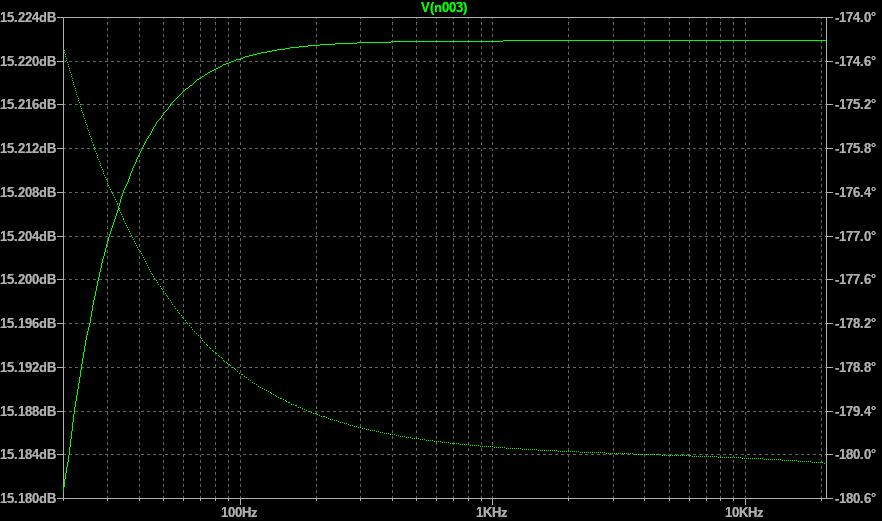
\includegraphics[scale=0.7]{frequency1.jpg}}
\caption{Frequency response without bypass capacitor}
\end{center}
\vspace{-30pt}
\end{figure}

\begin{figure}[h]
\begin{center}
\fbox{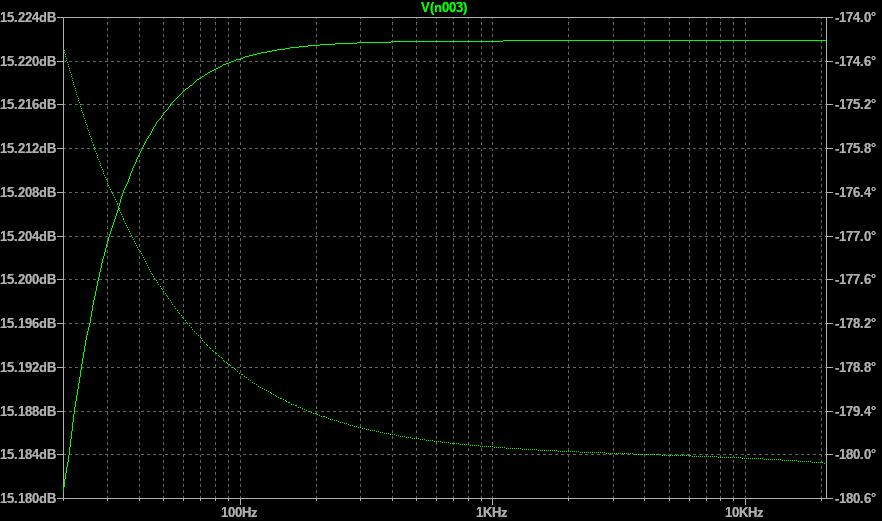
\includegraphics[scale=0.7]{frequency1.jpg}}
\caption{Frequency response without bypass capacitor}
\end{center}

\end{figure}
\vspace{-30pt}


 
\end{document}



